\chapter{Application Analysis} \label{ch:appanalysis}
This chapter will explore the application domain in the A$^3$ model described in section \vref{sec:a3model} and it is the domain marked on figure \vref{fig:a3app}. First, the basic principles of stereo vision will be described and then other aspects such as color versus grayscale etc. are analyzed. The results from this chapter will be used in chapter \vref{ch:req}.

\begin{figure}[ht!]
  \centering
  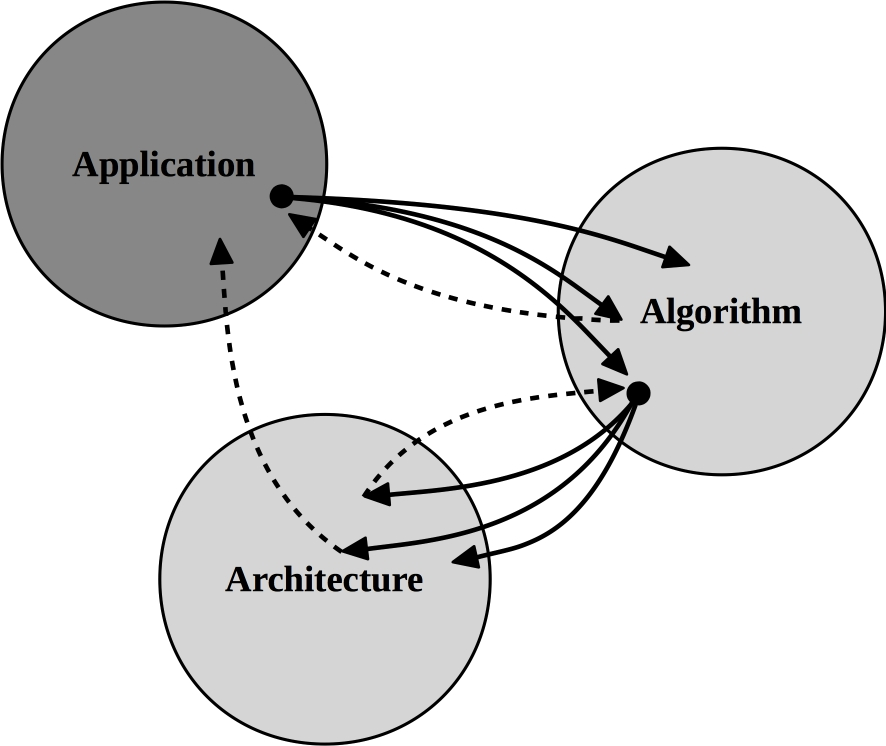
\includegraphics[scale=0.25]{figures/a3app}
  \caption{A$^3$ model with the application domain marked}
  \label{fig:a3app}
\end{figure}

\section{The Basic Principle of Stereo Vision}\label{sec:basicstereo}
A standard stereo vision setup consists of two similar cameras placed horizontally at a specified distance from each other. This distance is called the baseline. Figure \vref{fig:2cams_all} shows an example of this setup.\\
\begin{figure}[ht!]
  \centering
  \begin{subfigure}[t]{1\textwidth}
    \centering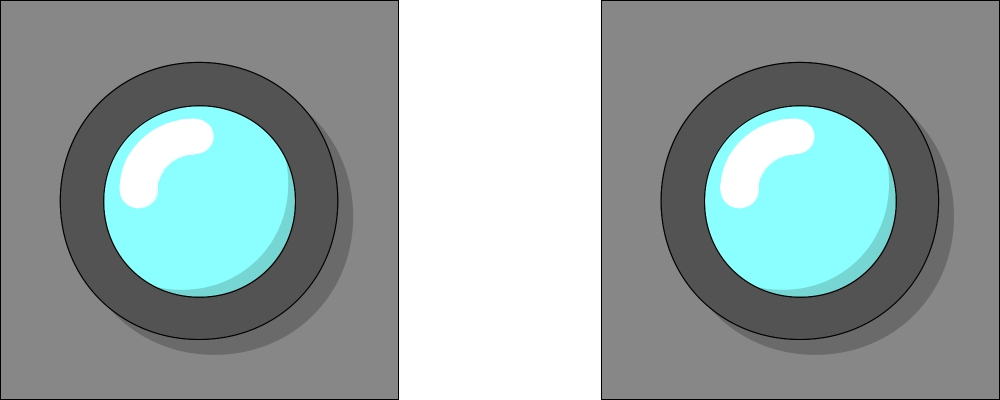
\includegraphics[width=0.3\textwidth]{figures/2cams_fro}
    \caption{Seen from the front\label{fig:2cams_fro}}
  \end{subfigure}\vspace{0.4cm}
  \begin{subfigure}[t]{1\textwidth}
    \centering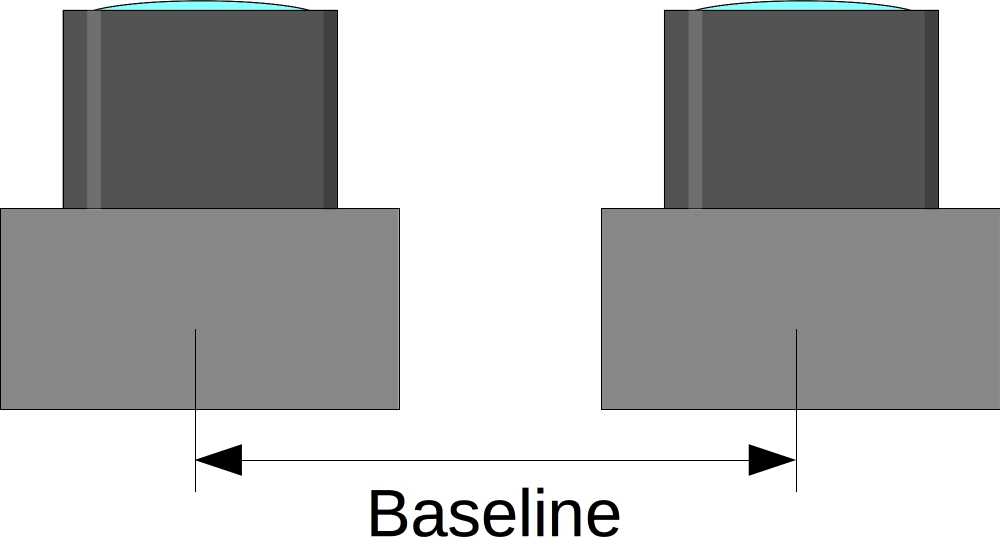
\includegraphics[width=0.3\textwidth]{figures/2cams_top}
    \caption{Seen from above\label{fig:2cams_top}}
  \end{subfigure}
  \caption{Illustration of a standard stereo vision setup\label{fig:2cams_all}}
\end{figure}

Figure \vref{fig:imgplane_all} shows how a scene is seen by the camera, is inverted in the optical center and projected onto the image sensor in the camera. The original image plane is located at the position of the image sensor but it is inverted compared to the scene captured. To simplify comparisons to the real world, an image plane can be placed opposite of the optical center at the same distance from the center and this image plane will not be inverted.

\begin{figure}[ht]
  \centering
  \begin{subfigure}[t]{0.3\textwidth}
    \centering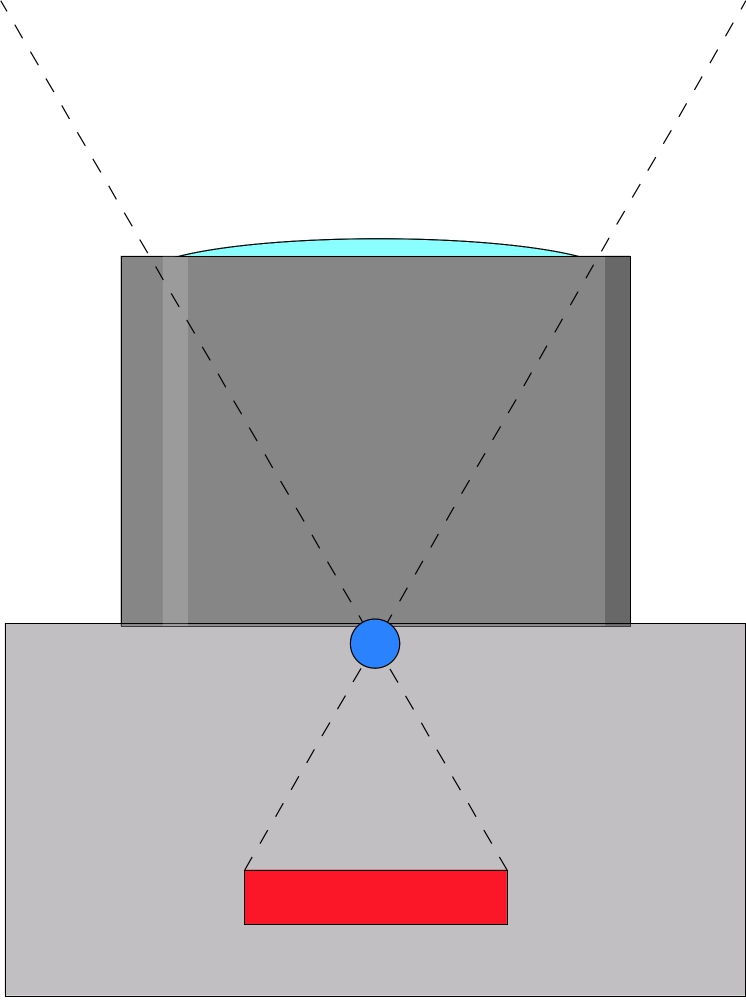
\includegraphics[height=4cm]{figures/imgplane_1.jpg}
    \caption{Location of the optical center and image sensor\label{fig:imgplane1}}
  \end{subfigure}\hspace{0.5cm}
  \begin{subfigure}[t]{0.3\textwidth}
    \centering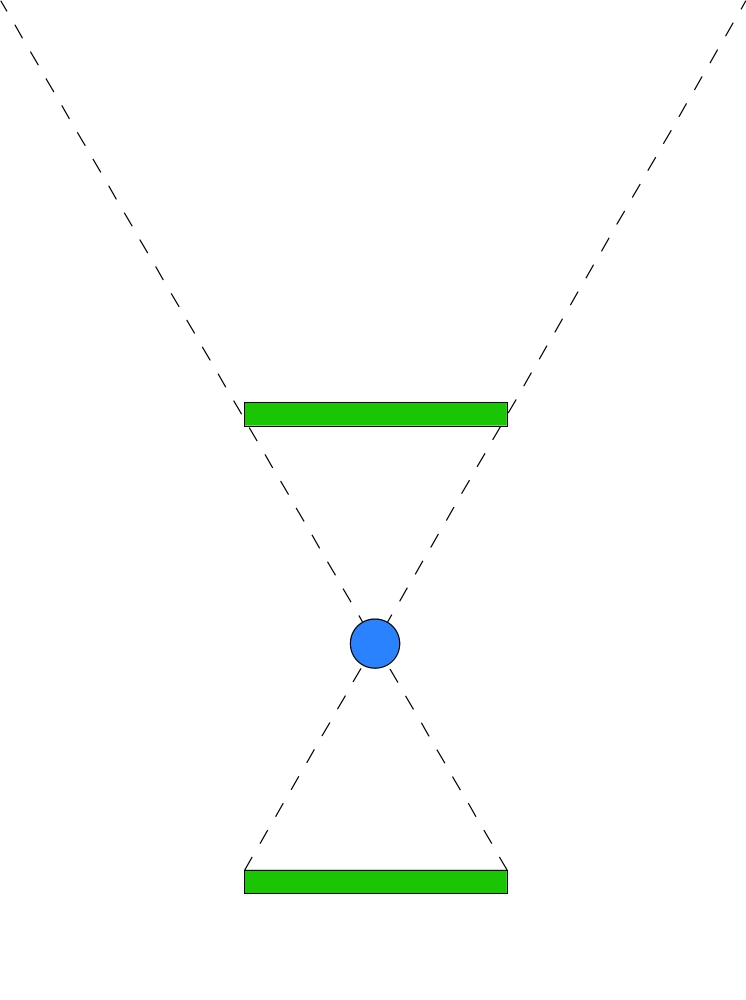
\includegraphics[height=4cm]{figures/imgplane_2}
    \caption{Location of the image plane\label{fig:imgplane2}}
  \end{subfigure}\hspace{0.5cm}
  \begin{subfigure}[t]{0.3\textwidth}
    \centering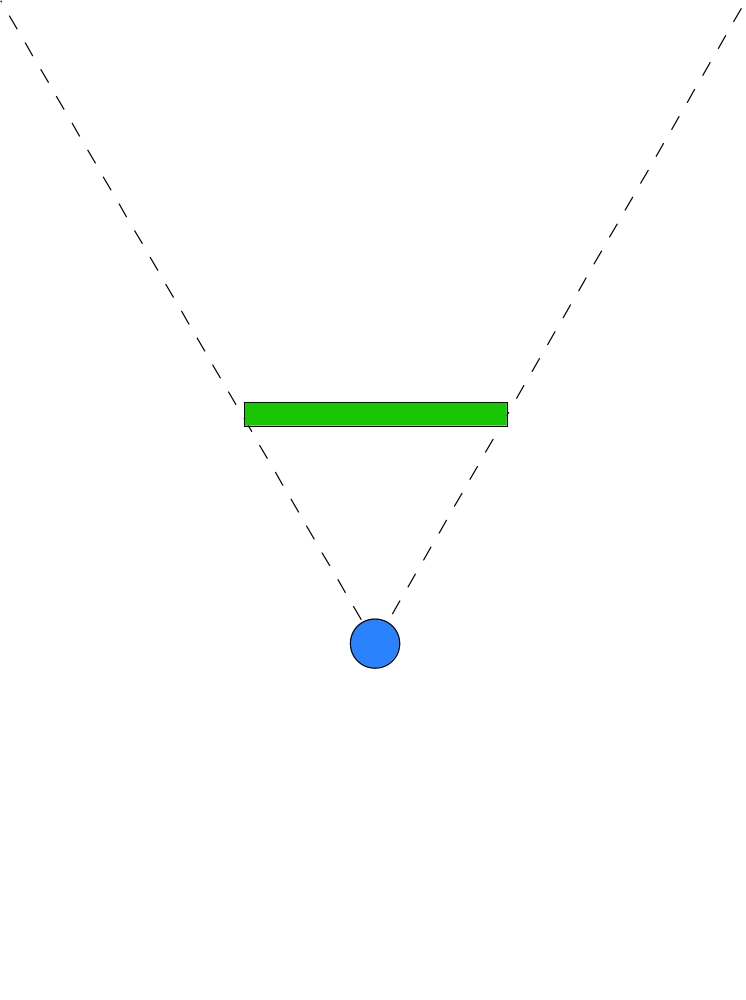
\includegraphics[height=4cm]{figures/imgplane_3}
    \caption{This illustration will be used to to explain disparity\label{fig:imgplane3}}
  \end{subfigure}
  \begin{subfigure}[t]{0.75\textwidth}
    \centering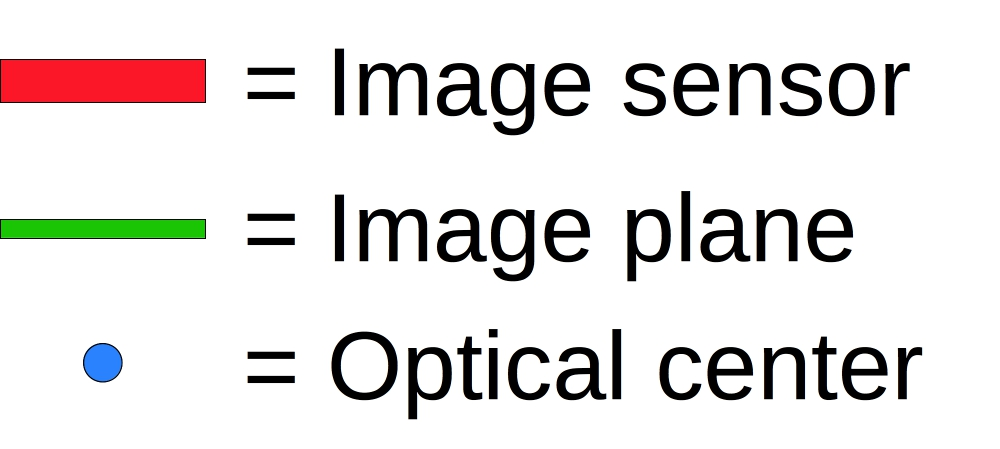
\includegraphics[width=0.4\textwidth]{figures/imgplane_legends}
  \end{subfigure}\hspace{0.5cm}
  \caption{Illustration of going from camera to image plane\label{fig:imgplane_all}}
\end{figure}

Figure \vref{fig:2points_1} shows that a single camera is not able to differentiate between two points at the same angle from the optical center at different distances. Figure \vref{fig:2points_2} illustrates how adding the second camera allows differentiating between the two points.

\begin{figure}[ht]
  \centering
  \begin{subfigure}[t]{0.45\textwidth}
    \centering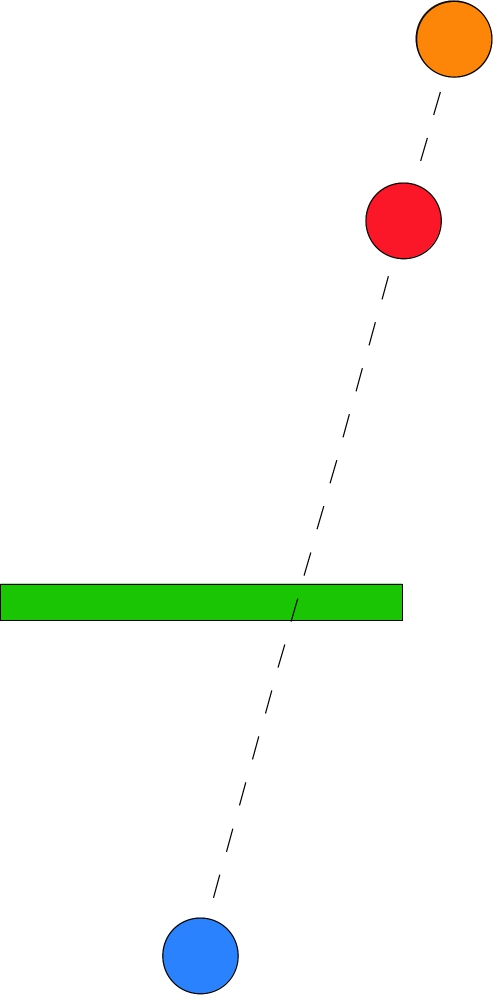
\includegraphics[height=4cm]{figures/2points_1}
    \caption{Seen from a single camera\label{fig:2points_1}}
  \end{subfigure}
  \begin{subfigure}[t]{0.45\textwidth}
    \centering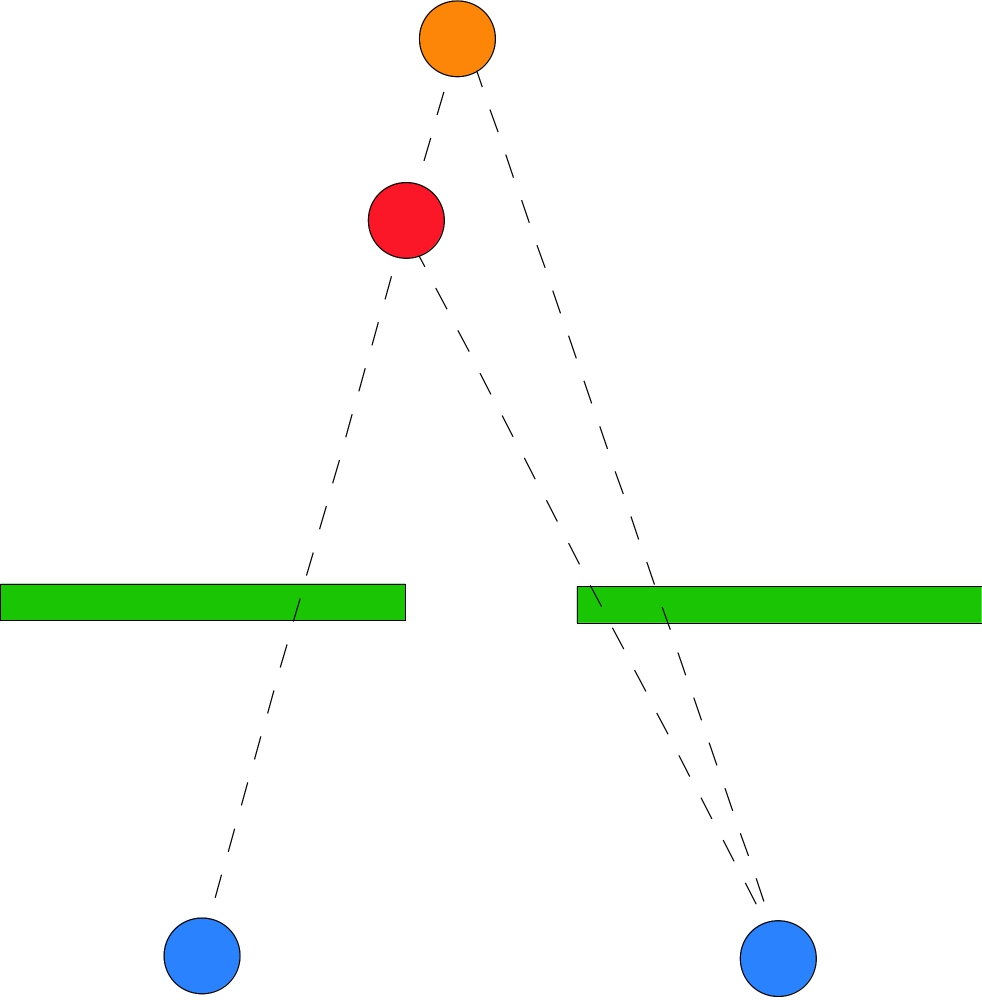
\includegraphics[height=4cm]{figures/2points_2}
    \caption{Seen from two cameras\label{fig:2points_2}}
  \end{subfigure}
  \caption{Example of two points in a scene at different depths\label{fig:2points_all}}
\end{figure}

Figure \vref{fig:dispall} shows how the distance to a point can be calculated from the difference in x-positions on the image plane (the disparity). Figure \vref{fig:disp_long} and \vref{fig:disp_short} shows how the disparity changes depending on the distance to the point. Figure \vref{fig:bfz_disp} shows the point in the scene (p), where line of sight crosses the image planes (i$_1$ and i$_2$) and the optical centers (c$_1$ and c$_2$). From these points two similarly angled  triangles can be created. One between p, i$_1$ and i$_2$ and the other triangle between p, c$_1$ and c$_2$. For similarly angled triangles the ratio between the height and the bottom width is the same for each triangle and hence the following equation can be formed:
\begin{flalign}
  && \frac{b}{z} &= \frac{L}{z-f} = \frac{b-(x_1-x_2)}{z-f} && \label{eq:disp_1}
\end{flalign}
$x_1-x_2$ is also called the disparity, $d$, and equation \vref{eq:disp_1} can be simplified:
\begin{flalign}
  && &z = \frac{b \cdot f}{d} && \label{eq:disp_final}
\end{flalign}

\begin{figure}[ht]
  \centering
  \begin{subfigure}[t]{0.3\textwidth}
    \centering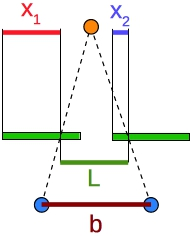
\includegraphics[scale=1]{figures/disparity_ex1.jpg}
    \caption{Disparity for a point far way\label{fig:disp_long}}
  \end{subfigure}\hspace{0.5cm}
  \begin{subfigure}[t]{0.3\textwidth}
    \centering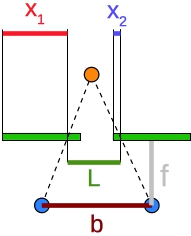
\includegraphics[scale=1]{figures/disparity_ex2}
    \caption{Disparity for point close\label{fig:disp_short}}
  \end{subfigure}\hspace{0.5cm}
  \begin{subfigure}[t]{0.3\textwidth}
    \centering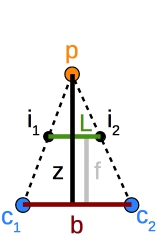
\includegraphics[scale=1]{figures/disparity_ex3}
    \caption{Illustration of triangles used for calculating the disparity\label{fig:bfz_disp}}
  \end{subfigure}
  \caption{Illustration of how to calculate depth from disparity\label{fig:dispall}}
\end{figure}

In equation \vref{eq:disp_final} $b$ and $f$ are known ($b$ is the baseline and $f$ is the focal length) hence only the disparity is needed to find $z$. So to find the distance to a point, the location of the point in the two images should be found and the displacement may be computed. \\

This explains the basics of stereo vision. The rest of this chapter will venture into other areas of stereo vision and describe the difficulties and solutions for each area.

\section{Epipolar Geometry}
Section \ref{sec:basicstereo} assumes that the stereo image planes are ideal, align exactly and being parallel with the baseline but in a real scenario the cameras will have small imperfections and variations which will make the image planes not perfectly align.\\
\begin{figure}[ht!]
  \centering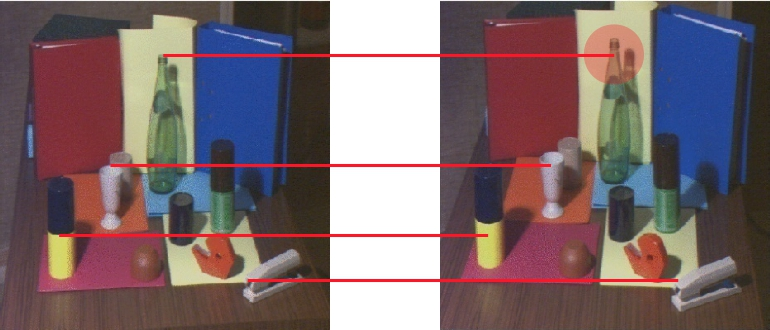
\includegraphics[height=5cm]{figures/nonrect.jpg}
  \caption{Non-rectified stereo pair\label{fig:nonrect} \cite{Mattoccia2013}}
\end{figure}
 
Figure \vref{fig:nonrect} shows a pair of stereo images. As seen when searching for a corresponding point in the second camera (e.g. the top of the bottle) then a 2D search area is needed. To simplify the search epipolar geometry can be used. \\

\begin{figure}[ht!]
  \centering
  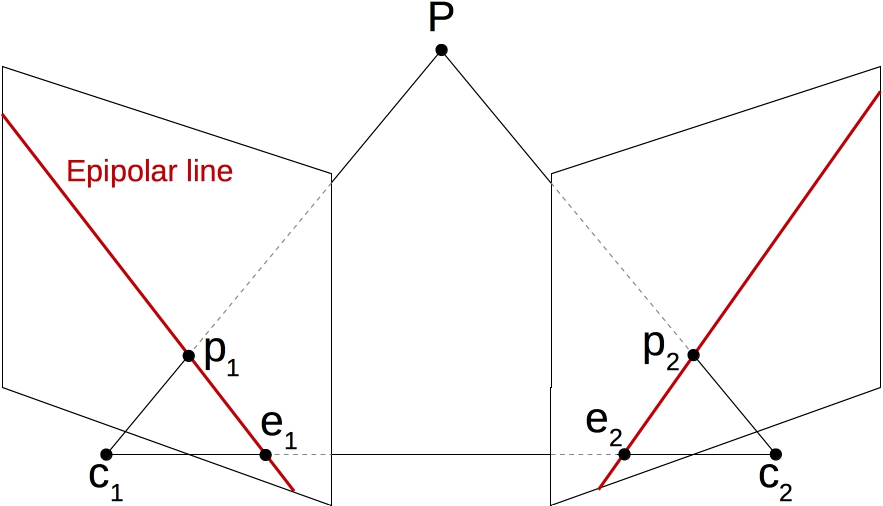
\includegraphics[height=4.5cm]{figures/epipolarsimple}
  \caption{Illustration of epipolar geometry}
  \label{fig:epipolarsimple}
\end{figure}

Epipolar geometry occurs when a scene is seen from two different views. Figure \vref{fig:epipolarsimple} illustrates epipolar geometry. An epipole is the projection, on one camera's image plane, of the optical center of the other camera and is noticed on figure \vref{fig:epipolarsimple} as the points where the line between the centers crosses the image planes. The red line going through p$_l$ (the projection of point P on the image plane) and the epipole is called an epipolar line and a corresponding epipolar line can be found on the other image plane. When searching for the corresponding point in the other image the search can be simplified from a 2D search to a 1D search along the epipolar line. To simplify the search further, the image can be rectified.\\

Rectification will transform the stereo images to remove lens distortion and make them into standard form. The standard form is helpful since all epipolar lines then will be horizontal and this simplifies the search for corresponding points to search along the x-axis. Figure \vref{fig:rect} shows the stereo image pair from figure \vref{fig:nonrect} but rectified. As seen, the corresponding points can now be found by following the horizontal lines or the x-axis.\\

\begin{figure}[ht!]
  \centering
  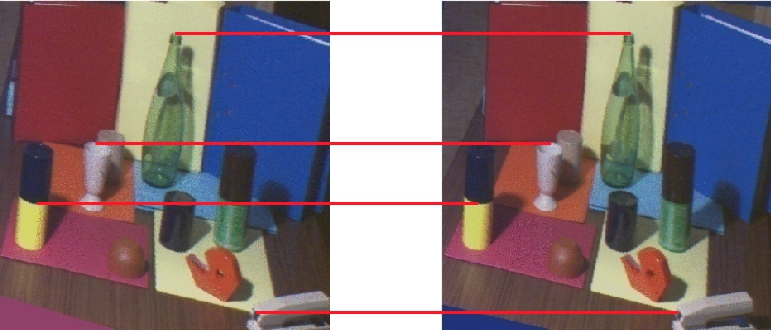
\includegraphics[height=4cm]{figures/rect}
  \caption{Rectified stereo pair\label{fig:rect} \cite{Mattoccia2013}}
\end{figure}

The issue with rectification is that it is difficult to get a perfect match with the stereo setup since every camera and its lens will be unique and require an all new manual calibration. HSA Systems theorizes that a system can be developed which instead of rectifying the image will find the epipolar lines for each epipole and feed this information to the stereo cameras.\\

In this project stereo image pairs from Middlebury Vision Test sets \cite{middlebury2016} will be used. These image pairs are rectified, and rectification of image will not be discussed further in this project.

\section{Color space and grayscale} \label{sec:color}
Colors can be represented in many different ways digitally using color spaces. Two of the most common color spaces are grayscale and RGB. Some studies have investigated what impact different color spaces can have on the result from a stereo vision algorithm.\\ 

For this project the impact of color spaces have not been studied but instead the findings in \cite{chambon2005colour} are used. This study describes the impact of color spaces on stereo matching by investigating 9 color spaces and 3 different methods. Table \vref{tab:colourres} shows parts of the results from \cite{chambon2005colour}. In this table the \textit{Measure} column is the algorithm used, \textit{Type} specifies whether it is grayscale (G) or color (C) with the best color space used, the \textit{Correct} column is the percentage of correct matches and \textit{Time} is the execution time. The article concludes that using color always results in better matching, but from table \vref{tab:colourres} it is seen that using grayscale lowers the execution time significantly compared to using color. In most cases without significant impact on the matching results.\\
\begin{table}
  \centering
  \begin{tabular}{l r | c | c }
    Measure & Type & Correct [\%] & Time\\
    \midrule
    Ncc & G & 52.3 & 52\\
          & C & 55.2 & 141\\
    \midrule
    D$_1$ & G & 49.5 & 63\\
               & C & 51.6 & 140\\
    \midrule
    PRATT & G & 29.1 & 86\\
              & C & 45.2 & 225\\
    \midrule
    ISC & G & 44.9 & 126\\
    & C & 52.6 & 245\\
    \midrule
    SMPD$_2$ & G & 49.9 & 569\\
    & C & 56.5 & 2109 \\
  \end{tabular}
  \caption{Part of table containing results from \cite{chambon2005colour}\label{tab:colourres}}
\end{table}

Since the main focus of the project is on a fast stereo vision algorithm and minding the results from table \vref{tab:colourres}, it is decided to use grayscale images if the tradeoff is not too significant.

\section{Disparity precision}\label{sec:disppre}
% New version
The depth resolution depends on different things in the stereo camera setup: the camera resolution, the focal length, the baseline etc. HSA Systems requires that the system has a \SI{\leq 5}{\milli\meter} depth resolution between \SI{0.5}{\meter} and \SI{1.5}{\meter}.\\
The sensor which will be used for a final product is a \textit{Sony IMX264} since this sensor is used in the company's smart camera products. This sensor has a resolution of 2464$\times$2056\label{req:camres}, a pixel size of \SI{3.45}{\micro\meter} \label{req:pixelsize} and a frame rate of 35.7 fps. Full specifications of the sensor can be found in \cite{sonyimx264-2016}. HSA Systems requires that the baseline is \SI{\leq 10}{\centi\meter}.\\
To calculate the precision equation \vref{eq:disp_final} is used. This equation is repeated here:
\begin{flalign}
 && z &= \frac{b\cdot f}{d} && \label{eq:disp_final2}
\end{flalign}
The disparity, $d$, of equation \vref{eq:disp_final2} is expressed in pixels and may be converted to mm by using the the pixel size ($p_{size}$) of the camera sensor. A focal length $f$ should be chosen so the scene at max distance will be $1.5\times$\SI{1,5}{\meter} \label{req:scenesize} and figure \vref{fig:scenesize} shows the relationship between scene size and focal length.\\

\begin{figure}[ht!]
  \centering
  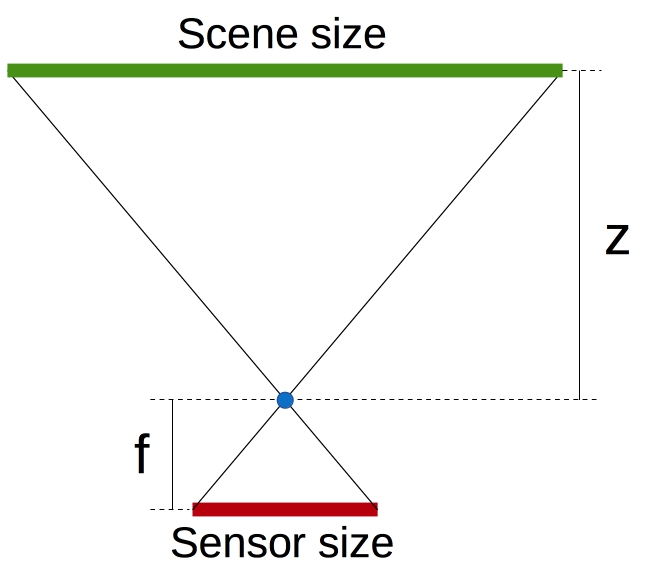
\includegraphics[scale=0.375]{figures/scenesize}
  \caption{Illustration of the relationship between sensor size, scene size, focal length and distance}
  \label{fig:scenesize}
\end{figure}
Since the two triangles in the figure are similar the focal length can be determined using:
\begin{equation}
 f = \frac{z \cdot s_{sensor}}{s_{scene}}
\end{equation}

Where $z$ is the distance, $s_{sensor}$ is the size of the sensor which depends on pixel size and resolution and $s_{scene}$ is the size of the scene. Since the camera resolution is not square a focal length for both horizontal and vertical scene size have to be calculated and the lowest focal length is chosen.
\begin{flalign}
  && f_h &= \frac{1500 \cdot 2464 \cdot 0.00345}{1500} = 8.5 mm && \\
  && f_v &= \frac{1500 \cdot 2056 \cdot 0.00345}{1500} = 7.09 mm && 
\end{flalign}
A focal length of \SI{7.09}{\milli\meter} is chosen\label{req:focallen} and this results in a scene size of $1798\times$\SI{1500}{\milli\meter}. With the baseline and focal length determined, it can be calculated when the disparity precision is \SI{\leq 5}{\milli\meter}.\\
The derivative of $z$ with respect to $d$ gives the precision at a specific disparity. 
\begin{equation}
  z' =  -\dfrac{b \cdot f}{p_{size} \times (d^2)} 
\end{equation}
Inserting the known values and the wanted precision the disparity $d$ is found to be $202,73$ but since the disparity is an integer this value should be rounded up to $203$. This results in a disparity precision of \SI{-4.99}{\milli\meter} and the distance where this precision is achieved is at \SI{1012.35}{\milli\meter}. This does not comply with the requirement from HSA Systems. Using sub-pixel refinement a precision of \SI{10}{\milli\meter} can be used to achieve the same precision. This precision is achieved at a disparity of $144$ and the precision is then \SI{-9.91}{\milli\meter} at the distance \SI{1427}{\milli\meter}. This still doesn't comply with the requirement. \\
To improve the precision further either the resolution, the baseline or the focal can be changed but each requires another requirement to fail. The resolution requires a new camera sensor. The baseline need to be at least \SI{11}{\milli\meter} larger. The focal length needs to at least \SI{0.73}{\milli\meter} higher but this results in a scene size of $1631 \times$\SI{1361}{\milli\meter}. \\

It is chosen to reduce the scene size to $1631 \times$\SI{1361}{\milli\meter} and use a focal length of \SI{7.82}{\milli\meter}. This results in a precision of  \SI{10}{\milli\meter} at  \SI{\approx 1500}{\milli\meter} so sub-pixel refinement has to be used. The resulting disparity range will be 303. Figure \vref{fig:dpre} shows the disparity precision at different distances with the chosen baseline, focal length, and sensor.
\begin{figure}[ht!]
  \centering
  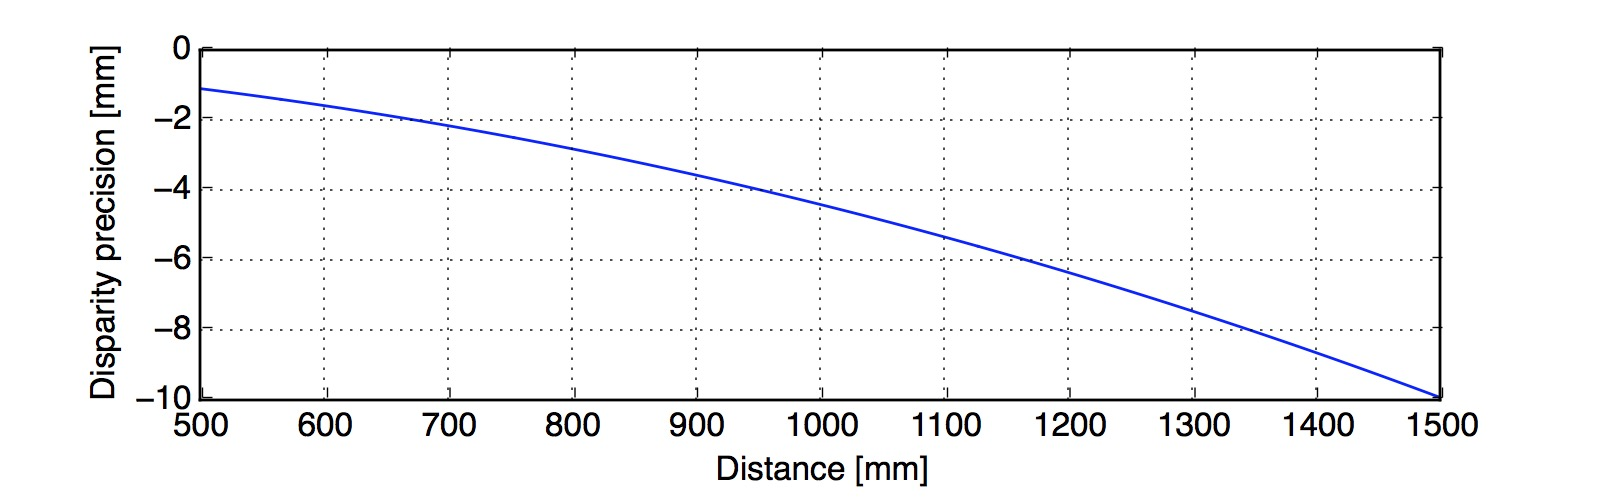
\includegraphics[width=0.9\textwidth]{figures/dpre}
  \caption{Disparity precision in the distance range \si{0.5}\SI{-1.5}{\meter}}
  \label{fig:dpre}
\end{figure}

\section{Occlusions}
Occlusions occur when an object closer to the camera setup entirely or partially blocks an object behind it. Figure \vref{fig:occlboth} illustrates two cylinders seen by a stereo camera setup where occlusion occurs. Figure \vref{fig:occltop} shows that the blue cylinder is only partially visible to the right camera because the red cylinder hides some of the blue cylinder (marked with red) while the left camera can see the whole of both cylinders. When searching for corresponding points in the occluded area issues occur. As illustrated by the arrow on figure \vref{fig:occl2view}, the edge of the blue cylinder can not be found and it will result in calculating a wrong disparity value. \\

\begin{figure}[ht]
  \centering
  \begin{subfigure}[t]{0.45\textwidth}
    \centering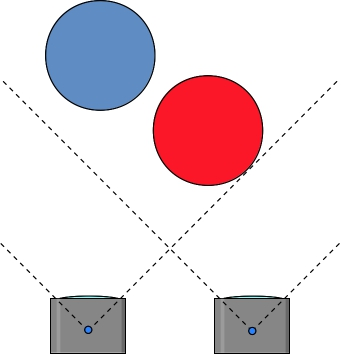
\includegraphics[scale=0.4]{figures/occltop.jpg}
    \caption{Stereo camera setup with two cylinders in the scene seen from above\label{fig:occltop}}
  \end{subfigure}\hspace{0.5cm}
  \begin{subfigure}[t]{0.45\textwidth}
    \centering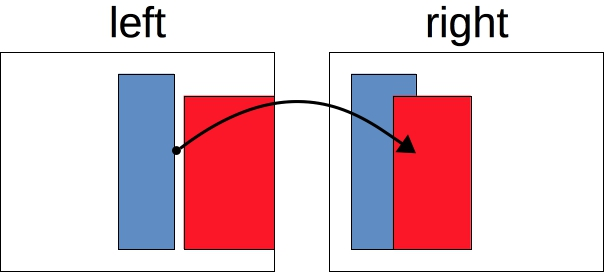
\includegraphics[scale=0.4]{figures/occl2view}
    \caption{Image seen by each camera in figure \vref{fig:occltop}\label{fig:occl2view}}
  \end{subfigure}
  \caption{Illstration of occlusions\label{fig:occlboth}}
\end{figure}

There exist different types of occlusions: partial occlusions, self-occlusions, border occlusions and total occlusions. Partial occlusions are when an object is only partially obstructed as seen on figure \vref{fig:occlboth}. Self-occlusion occurs on round surfaces such as faces, and balls and as seen on figure \vref{fig:occlself} the surfaces marked with red can be seen by one camera but not the other camera. Border occlusions occur when an object or part of an object is outside the view of one camera but not the other camera as seen with the blue object on figure \ref{fig:occltb}. Total occlusion is when an object is completely hidden by an object in the view of one camera but not in the view of the other camera and an example of this is seen with the red object on figure \vref{fig:occltb}.\\

\begin{figure}[ht!]
  \centering
  \begin{subfigure}[t]{0.45\textwidth}
    \centering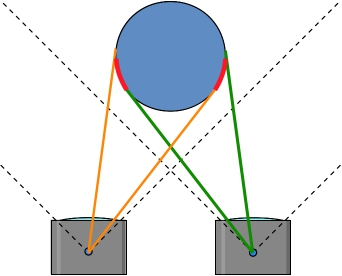
\includegraphics[scale=0.4]{figures/occlself.jpg}
    \caption{Illustartion of self occlusion seen from above\label{fig:occlself}}
  \end{subfigure}\hspace{0.5cm}
  \begin{subfigure}[t]{0.45\textwidth}
    \centering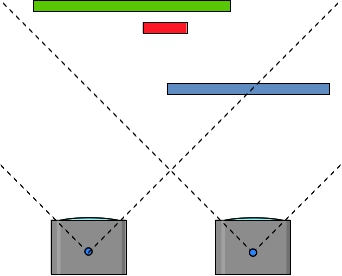
\includegraphics[scale=0.4]{figures/occltotalborder}
    \caption{Illustration of total and border occlusions seen from above\label{fig:occltb}}
  \end{subfigure}
  \caption{Illustration of different types of occlusions\label{fig:occltypes}}
\end{figure}

Occluded points can be found by running stereo matching again but switching which camera is used as the reference and then compare the disparity values found for each direction. When occluded areas are found these can be filled using different methods. For this project the findings from \cite{huq2013occlusion} is used which will be described in section \vref{sec:nda} to \vref{sec:sls}. The methods will only be briefly described in this report and a more thorough description can be found in \cite{huq2013occlusion}. All these methods assume that the stereo matching is using the left image as reference i.e. the points in the left image are searched for in the right image. 

\subsection{Neighbor's Disparity Assignment (NDA)}\label{sec:nda}
This is one of the simpler methods to fill occlusions. It functions by selecting an occluded point, $p_L$, then finds then nearest non-occluded point, $q_L$, to the left when filling non-border occlusion. With border occlusion, the nearest point to the right is found instead. This method assumes that this non-occluded point is part of the same surface as the occluded point (this can be seen on figure \ref{fig:occlboth}) and the disparity value from $q_L$ can be assigned to $p_L$. This method has some issues. In cases of total occlusions (see figure \ref{fig:occltb}) wrong disparity values will be given to the total occluded object since it is not a part of the nearest surface with non-occluded points to the left. In cases with self-occlusions the occluded area should have disparity values close to the disparity values of the non-occluded points to the right (This will be the area of the surface which is in view of both cameras) but using NDA will give the occluded area disparity values corresponding to the background.

\subsection{Diffusion in Intensity Space (DIS)}
This method is inspired by diffusion. Diffusion is the movement of molecules or atoms from a high concentration region to a low concentration region. \\

After detecting occluded regions with cross-checking during stereo matching, the diffusion energy for the region is approximated. This method is dependent on the stereo matching algorithm because it uses the energy from the last iteration to determine initial diffusion energy for the area. But a change to the method can be made to make it independent from the stereo matching. The initial diffusion energy will be 0. Then the diffusion energy for an occluded point  $E(p_L)$ is calculated by basically integrating the energies of non-occluded points with the same disparity value in the neighborhood of the occluded point $p_L$. The disparity value which results in the lowest diffusion energy will be given to $p_L$. This is repeated for each occluded point until every point have been filled.

\subsection{Weighted Least Squares (WLS)}
In this method, all the non-occluded and filled occluded neighbors in a neighborhood around the occluded point is considered valid points and is used as control points in interpolation. But since the neighborhood contains both foreground points and background points and the occluded point is expected to be a part of the background then the background points should have higher influence than foreground points. \\

Therefore a weighted least square problem is set up where the residual error term is weighted so non-occluded points belonging to foreground objects will have a lower influence on the least square problem than points belonging to the background. To distinguish between foreground points and background points it can be assumed that the color intensity between objects is significantly different. \\

\subsection{Segmentation-based Least Squares (SLS)}\label{sec:sls}
This method is an alteration of the WLS method. The biggest difference between WLS and SLS is that SLS only uses non-occluded points as control points. The control points is a subset of the non-occluded neighboring points. The control points are segmented from the neighborhood by applying different constraints: visibility constraint, disparity gradient constraint, and color similarity cues.\\

First find occluded points which have at least one non-occluded neighboring point. Then these points are sorted by a priority which is found by checking the homogeneity i.e color similarity between the occluded point, $p_L$ and the neighboring non-occluded points.\\

When the occluded point with the highest priority is found then some initial control points from the neighborhood are needed. First only points from the background is wanted therefore only points in the neighborhood which have a disparity value lower than the foreground. The nearest non-occluded point to the left of the occluded point is assumed to be part of the background, $l_{p_{Lb}}$, and the nearest non-occluded point to the right is assumed to be part of the foreground, $l_{p_{Lf}}$. But narrow objects in the foreground will make the non-occluded point on either side of the occluded area be part of the background. So some constraints are setup to get all the background points. The constraints will find every point which has a disparity value close to the background points $l_{p_{Lb}}$ or lower than the foreground points
$l_{p_{Lf}}$.\\

All points in the neighborhood, which satisfies these constraints, is assumed to be part of the background but might contain points from multiple background surfaces. It is assumed, from looking at the data sets from \cite{middlebury2016}, that the neighborhood only contains points from either one background surface or two background surfaces. If the difference between highest and lowest value is too high then this new neighborhood contains two objects and have to be divided into two neighborhoods. This is done by grouping all points with disparity values close to the lowest disparity and all points with disparity values close to the highest disparity. Then it can be determined which group the occluded point belongs to by looking at color distance to each group. \\

With these control points found a least square problem can be set up using these control points for finding the disparity value of the occluded point.

\section{Occlusions filling result}
In \cite{huq2013occlusion} it is found that SLS gives the best result followed by DIS, NDA, and WLS but the runtime SLS is slower than NDA and WLS and faster than DIS. Since the project focuses on implementing a fast stereo algorithm and focuses more on the stereo algorithm itself, NDA is chosen as the method to fill occlusions since it is the better performing of the two faster methods. 

\section{Wrap-up}
To conclude this chapter the findings for each area in stereo vision will be examined and it will be specified which solution will be used from this point.
\subsection*{Rectification of Images}
This project will not delve further into the subject of rectification. Instead data sets from \cite{middlebury2016}, will be used in this project as they are already rectified.

\subsection*{Color Space}
The result from \cite{chambon2005colour} shows that color spaces in most cases are slightly better than using grayscale images but the computational complexity is much higher. This result depends on the algorithm used therefore when an algorithm has been chosen a test should check if grayscale images perform much worse than using color images and what the impact on run time is.

\subsection*{Resolution and Disparity Precision}
To have a disparity precision of 2 mm at 1500 mm using \textit{Imaging Source DMK 72BUC02} cameras with a resolution of 2592$\times$1944 and a pixel size of 2.2 \si{\micro\meter} a lens with a focal length of 10 mm should be used together with subpixel refinement.

\subsection*{Occlusions}
4 different methods to fill occlusions were described and from these NDA is chosen since it is the better performing of the two faster algorithms.